% defer/refcnt.tex
% mainfile: ../perfbook.tex
% SPDX-License-Identifier: CC-BY-SA-3.0

\section{Reference Counting}
\label{sec:defer:Reference Counting}
%
\epigraph{I am never letting you go!}{Unknown}

\begin{listing}[tbp]
\input{CodeSamples/defer/route_refcnt@lookup.fcv}
\caption{Reference-Counted Pre-BSD Routing Table Lookup (BUGGY!!!)}
\label{lst:defer:Reference-Counted Pre-BSD Routing Table Lookup}
\end{listing}

\begin{listing}[tbp]
\input{CodeSamples/defer/route_refcnt@add_del.fcv}
\caption{Reference-Counted Pre-BSD Routing Table Add\slash Delete (BUGGY!!!)}
\label{lst:defer:Reference-Counted Pre-BSD Routing Table Add/Delete}
\end{listing}

레퍼런스 카운팅은 객체가 너무 이르게 메모리 해제되는 걸 방지하기 위해 참조 수를
기록합니다.
그것으로서, 이것은 최소한 1960년대 Weizenbaum 의
논문~\cite{Weizenbaum:1963:SLP:367593.367617} 까지 거슬러 올라가는 길고
영광스런 사용 역사를 가졌습니다.
Weizenbaum 은 레퍼런스 카운팅을 그게 이미 잘 알려진 것처럼 이야기 했으니,
1950년대나 심지어 1940년대까지 거슬러 올라갈 수도 있습니다.
그리고 어쩌면 그보다 심지어 더 나아가서, 크고 위험한 기계를 수리하는 사람들은
패드락을 통해 구현된 기계적 레퍼런스 카운팅 기법을 오랫동안 사용해 왔습니다.
기계에 들어가기 전에, 각 작업자는 패드락을 기계의 on/off 스위치 위에서 잠궈서
이 기계가 작업자가 안에 들어가 있는 사이에 켜지는 걸 방지했습니다.
따라서 레퍼런스 카운팅은 Pre-BSD 라우팅의 동시적 구현을 위한 시간으로 증명된
좋은 후보가 될 수 있습니다.

\iffalse

Reference counting tracks the number of references to a given object in
order to prevent that object from being prematurely freed.
As such, it has a long and honorable history of use dating back to
at least an early 1960s Weizenbaum
paper~\cite{Weizenbaum:1963:SLP:367593.367617}.
Weizenbaum discusses reference counting as if it was already well-known,
so it likely dates back to the 1950s or even to the 1940s.
And perhaps even further, given that people repairing large dangerous
machines have long used a mechanical reference-counting technique
implemented via padlocks.
Before entering the machine, each worker locks a padlock onto the
machine's on/off switch, thus preventing the machine from being powered
on while that worker is inside.
Reference counting is thus an excellent time-honored candidate for a
concurrent implementation of Pre-BSD routing.

\fi

그런 이유로,
Listing~\ref{lst:defer:Reference-Counted Pre-BSD Routing Table Lookup}
은 데이터 구조와 \co{route_lookup()} 함수를 보이고
Listing~\ref{lst:defer:Reference-Counted Pre-BSD Routing Table Add/Delete}
은 \co{route_add()} 와 \co{route_del()} 함수를 보입니다 (모두
\path{route_refcnt.c} 에 있습니다).
이 알고리즘들은
Listing~\ref{lst:defer:Sequential Pre-BSD Routing Table}
에 보인 순차적 알고리즘과 상당히 비슷하므로 차이점만 이야기 하겠습니다.

\iffalse

To that end,
Listing~\ref{lst:defer:Reference-Counted Pre-BSD Routing Table Lookup}
shows data structures and the \co{route_lookup()} function and
Listing~\ref{lst:defer:Reference-Counted Pre-BSD Routing Table Add/Delete}
shows the \co{route_add()} and \co{route_del()} functions
(all at \path{route_refcnt.c}).
Since these algorithms are quite similar to the sequential algorithm
shown in
Listing~\ref{lst:defer:Sequential Pre-BSD Routing Table},
only the differences will be discussed.

\fi

\begin{fcvref}[ln:defer:route_refcnt:lookup:entry]
Listing~\ref{lst:defer:Reference-Counted Pre-BSD Routing Table Lookup}
부터 시작해 보자면, 라인~\lnref{refcnt} 는 실제 레퍼런스 카운터를 추가하고,
라인~\lnref{freed} 는 메모리 해제 후 사용 체크 필드인 \co{->re_freed} 를
추가하고, 라인~\lnref{routelock} 은 동시적 업데이트를 동기화 하는데 사용할
\co{routelock} 을 추가하며,
\end{fcvref}
\begin{fcvref}[ln:defer:route_refcnt:lookup:re_free]
\clnrefrange{b}{e} 는 \co{->re_freed} 를 세팅하고 메모리 해제 후 사용 버그를
체크하기 위한 \co{route_lookup()} 을 활성화 시키는 \co{re_free()} 를
추가합니다.
\end{fcvref}
\begin{fcvref}[ln:defer:route_refcnt:lookup:lookup]
\co{route_lookup()} 내에서, \clnrefrange{relprev:b}{relprev:e} 는 앞 원소의
레퍼런스 카운트를 해제하고 그 카운트가 0이 되면 메모리 해제시키며
\clnrefrange{acq:b}{acq:e} 는 새 원소의 레퍼런스를 획득하며,
라인~\lnref{check_uaf} 와~\lnref{abort} 는 메모리 해제 후 사용 체크를
수행합니다.
\end{fcvref}

\iffalse

\begin{fcvref}[ln:defer:route_refcnt:lookup:entry]
Starting with
Listing~\ref{lst:defer:Reference-Counted Pre-BSD Routing Table Lookup},
line~\lnref{refcnt} adds the actual reference counter,
line~\lnref{freed} adds a \co{->re_freed}
use-after-free check field,
line~\lnref{routelock} adds the \co{routelock} that will
be used to synchronize concurrent updates,
\end{fcvref}
\begin{fcvref}[ln:defer:route_refcnt:lookup:re_free]
and \clnrefrange{b}{e} add \co{re_free()}, which sets
\co{->re_freed}, enabling \co{route_lookup()} to check for
use-after-free bugs.
\end{fcvref}
\begin{fcvref}[ln:defer:route_refcnt:lookup:lookup]
In \co{route_lookup()} itself,
\clnrefrange{relprev:b}{relprev:e} release the reference
count of the prior element and free it if the count becomes zero,
and \clnrefrange{acq:b}{acq:e} acquire a reference on the new element,
with lines~\lnref{check_uaf}
and~\lnref{abort} performing the use-after-free check.
\end{fcvref}

\fi

\QuickQuiz{
	메모리 해제 후 사용 체크를 왜 신경쓰죠?

	\iffalse

	Why bother with a use-after-free check?

	\fi

}\QuickQuizAnswer{
	버그를 발견할 확률을 높이기 위해서입니다.
	한 타입의 구조체를 할당하고 해제하기만 하는 작은 고문 테스트 프로그램
	(\path{routetorture.h}) 는 놀랍도록 많은 양의 메모리 해제 후 사용
	문제를 제어할 수 있습니다.
	버그를 찾는 확률을 높이는 것의 중요성에 대해 더 많은 내용을 위해
	페이지~\pageref{fig:debugging:Number of Tests Required for 99 Percent Confidence Given Failure Rate}
	의
	Figure~\ref{fig:debugging:Number of Tests Required for 99 Percent Confidence Given Failure Rate}
	와
	페이지~\pageref{sec:debugging:Hunting Heisenbugs}
	에서 시작하는
	Section~\ref{sec:debugging:Hunting Heisenbugs}
	의 관련된 이야기를 보시기 바랍니다.

	\iffalse

	To greatly increase the probability of finding bugs.
	A small torture-test program
	(\path{routetorture.h}) that allocates and frees only
	one type of structure can tolerate a surprisingly
	large amount of use-after-free misbehavior.
	See Figure~\ref{fig:debugging:Number of Tests Required for 99 Percent Confidence Given Failure Rate}
	on page~\pageref{fig:debugging:Number of Tests Required for 99 Percent Confidence Given Failure Rate}
	and the related discussion in
	Section~\ref{sec:debugging:Hunting Heisenbugs}
	starting on
	page~\pageref{sec:debugging:Hunting Heisenbugs}
	for more on the importance
	of increasing the probability of finding bugs.

	\fi

}\QuickQuizEnd

\begin{fcvref}[ln:defer:route_refcnt:add_del]
Listing~\ref{lst:defer:Reference-Counted Pre-BSD Routing Table Add/Delete}
에서, 라인~\lnref{acq1}, \lnref{rel1}, \lnref{acq2}, \lnref{rel2},
그리고~\lnref{rel3} 는 동시적 업데이트들을 동기화 시키기 위한 락킹을 넣습니다.
라인~\lnref{init:freed} 은 메모리 해제 후 사용 체크 필드인 \co{->re_free}  를
초기화 하고 마지막으로 \clnrefrange{re_free:b}{re_free:e} 는 레퍼런스 카운트의
값이 0일 때 \co{re_free()} 를 호출합니다.
\end{fcvref}

\iffalse

\begin{fcvref}[ln:defer:route_refcnt:add_del]
In Listing~\ref{lst:defer:Reference-Counted Pre-BSD Routing Table Add/Delete},
lines~\lnref{acq1}, \lnref{rel1}, \lnref{acq2}, \lnref{rel2},
and~\lnref{rel3} introduce locking to synchronize
concurrent updates.
Line~\lnref{init:freed} initializes the \co{->re_freed} use-after-free-check field,
and finally \clnrefrange{re_free:b}{re_free:e} invoke
\co{re_free()} if the new value of
the reference count is zero.
\end{fcvref}

\fi

\QuickQuiz{
	Listing~\ref{lst:defer:Reference-Counted Pre-BSD Routing Table Add/Delete}
	의 \co{route_del()} 은 메모리 해제될 원소로의 횡단을 보호하기 위해서는
	레퍼런스 카운트를 사용하지 않나요?

	\iffalse

	Why doesn't \co{route_del()} in
	Listing~\ref{lst:defer:Reference-Counted Pre-BSD Routing Table Add/Delete}
	use reference counts to
	protect the traversal to the element to be freed?

	\fi

}\QuickQuizAnswer{
	이 횡단은 이미 락을 통해 보호되고 있어서 추가적 보호가 필요하지 않기
	때문입니다.

	\iffalse

	Because the traversal is already protected by the lock, so
	no additional protection is required.

	\fi

}\QuickQuizEnd

\begin{figure}[tb]
\centering
\resizebox{2.5in}{!}{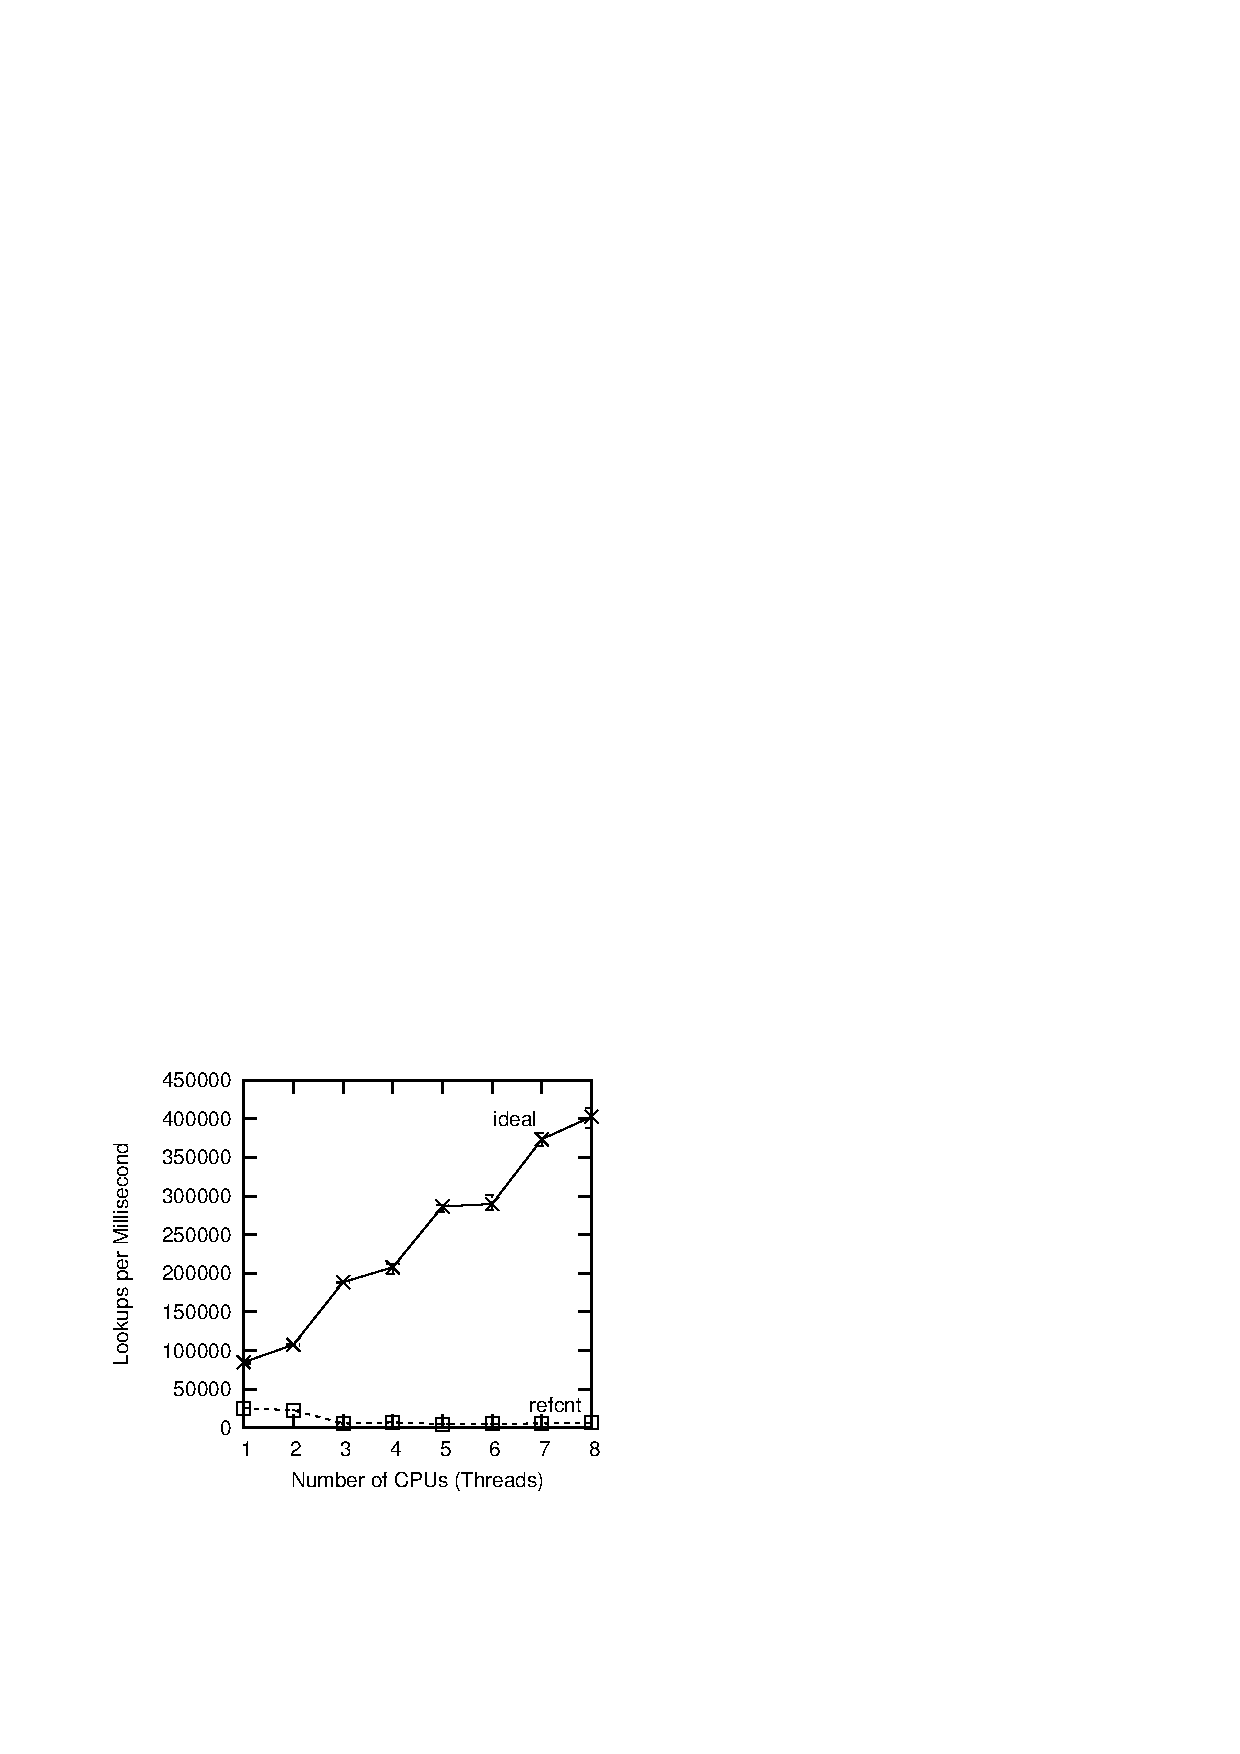
\includegraphics{CodeSamples/defer/perf-refcnt}}
\caption{Pre-BSD Routing Table Protected by Reference Counting}
\label{fig:defer:Pre-BSD Routing Table Protected by Reference Counting}
\end{figure}

Figure~\ref{fig:defer:Pre-BSD Routing Table Protected by Reference Counting}
는 총 448개 하드웨어 쓰레드를 갖는 여덟개 소켓의 소켓당 28 코어를 갖는
하이퍼쓰레드 기반 2.1\,GHz x86 시스템에서의 열개 원소를 갖는 리스트의 읽기 전용
워크로드에서의 레퍼런스 카운팅의 성능과 확장성을 보입니다
(\path{hps.2019.12.02a/lscpu.hps}).
``ideal'' 트레이스는
Listing~\ref{lst:defer:Sequential Pre-BSD Routing Table} 에 보인 순차적 코드를
통해 만들어졌는데, 이건 읽기 전용 워크로드이기 때문에 동작합니다.
레퍼런스 카운팅의 성능은 참담하고 그 확장성은 그보다 더한데, x 축에 구분할 수
없는 ``refcnt'' 트레이스로 보여져 있습니다.
Chapter~\ref{chp:Hardware and its Habits} 에서의 시각에 따르면 이건 놀랍지
않습니다:
레퍼런스 카운트 획득과 해제는 그게 사용되지 않았다면 읽기만 이루어졌을
워크로드에 빈번한 공유 메모리 쓰기를 추가하여, 물리 법칙으로부터 상당한 보복을
일으킵니다.
원래 그래야 하듯, 세상의 모든 희망적 생각들이 현대의 디지털 전자장치에 사용되는
빛의 속도를 높이거나 원자의 크기를 줄이지는 않습니다.

\iffalse

Figure~\ref{fig:defer:Pre-BSD Routing Table Protected by Reference Counting}
shows the performance and scalability of reference counting on a
read-only workload with a ten-element list running on an eight-socket
28-core-per-socket hyperthreaded 2.1\,GHz x86 system with a total of
448 hardware threads (\path{hps.2019.12.02a/lscpu.hps}).
The ``ideal'' trace was generated by running the sequential code shown in
Listing~\ref{lst:defer:Sequential Pre-BSD Routing Table},
which works only because this is a read-only workload.
The reference-counting performance is abysmal and its scalability even
more so, with the ``refcnt'' trace indistinguishable from the x-axis.
This should be no surprise in view of
Chapter~\ref{chp:Hardware and its Habits}:
The reference-count acquisitions and releases have added frequent
shared-memory writes to an otherwise read-only workload, thus
incurring severe retribution from the laws of physics.
As well it should, given that all the wishful thinking in the world
is not going to increase the speed of light or decrease the size of
the atoms used in modern digital electronics.

\fi

\QuickQuizSeries{%
\QuickQuizB{
	Figure~\ref{fig:defer:Pre-BSD Routing Table Protected by Reference Counting}
	의 224 CPU 에서의 ``ideal'' 선의 끊어짐은 무엇 때문인가요?
	곧은 선이어야 하지 않아요?

	\iffalse

	Why the break in the ``ideal'' line  at 224 CPUs in
	Figure~\ref{fig:defer:Pre-BSD Routing Table Protected by Reference Counting}?
	Shouldn't it be a straight line?

	\fi

}\QuickQuizAnswerB{
	그 끊어짐은 하이퍼쓰레딩 때문입니다.
	이 시스템에서, 소켓 내의 각 코어의 첫번째 하드웨어 쓰레드는 연속적인
	CPU 숫자를 가지며, 이 숫자는 다른 소켓의 각 코어의 첫번째 하드웨어들로
	이어지고, 마지막으로 모든 소켓의 각 코어의 두번째 하드웨어 쓰레드로
	이어집니다.
	이 시스템에서, CPU 숫자 0--27 는 이 첫번째 소켓의 28개 코어의 첫번째
	하드웨어 쓰레드이고, 숫자 28--55 는 두번째 소켓의 28개 코어의 첫번째
	하드웨어 쓰레드이며, 그렇게 이어져서 196--223 의 숫자는 여덟번째 소켓의
	28개 코어의 첫번째 하드웨어 쓰레드입니다.
	따라서 CPU 숫자 224-251 는 첫번째 소켓의 28개 코어의 두번째 하드웨어
	쓰레드이고 252--279 는 두번째 소켓의 28개 코어의 두번째 하드웨어
	쓰레드이며, 그렇게 이어져서 420--447 까지는 여덟번째 소켓의 28개 코어의
	두번째 하드웨어 쓰레드입니다.

	이게 왜 문제일까요?

	\iffalse

	The break is due to hyperthreading.
	On this particular system, the first hardware thread in each
	core within a socket have consecutive CPU numbers,
	followed by the first hardware threads in each core for the
	other sockets,
	and finally followed by the second hardware thread in each core
	on all the sockets.
	On this particular system, CPU numbers 0--27 are the first
	hardware threads in each of the 28 cores in the first socket,
	numbers 28--55 are the first hardware threads in each of the
	28 cores in the second socket, and so on, so that numbers 196--223
	are the first hardware threads in each of the 28 cores in
	the eighth socket.
	Then CPU numbers 224--251 are the second hardware threads in each 
	of the 28 cores of the first socket, numbers 252--279 are the
	second hardware threads in each of the 28 cores of the second
	socket, and so on until numbers 420--447 are the second hardware
	threads in each of the 28 cores of the eighth socket.

	Why does this matter?

	\fi

	코어의 두개 하드웨어 쓰레드는 자원을 공유하며, 이 워크로드는 하나의
	하드웨어 쓰레드가 그 코어의 자원의 절반 이상을 소비하게 하는 것
	같습니다.
	따라서, 해당 코어의 두번째 하드웨어 쓰레드를 추가하는 것은 희망하는
	것보다 자원을 덜 추가하는 게 됩니다.
	다른 워크로드는 각 코어의 두번째 하드웨어 쓰레드에서 더 큰 이득을 얻을
	수도 있겠습니다만, 하드웨어와 워크로드 양쪽의 세부사항에 의존적일
	겁니다.

	\iffalse

	Because the two hardware threads of a given core share resources,
	and this workload seems to allow a single hardware thread to
	consume more than half of the relevant resources within its core.
	Therefore, adding the second hardware thread of that core adds
	less than one might hope.
	Other workloads might gain greater benefit from each core's
	second hardware thread, but much depends on the details of both
	the hardware and the workload.

	\fi

}\QuickQuizEndB
%
\QuickQuizE{
	Figure~\ref{fig:defer:Pre-BSD Routing Table Protected by Reference Counting}
	의 refcnt 트레이스는 최소한 x-axis 에서 좀 떨어져야 하는 거 아닌가요???

	\iffalse

	Shouldn't the refcnt trace in
	Figure~\ref{fig:defer:Pre-BSD Routing Table Protected by Reference Counting}
	be at least a little bit off of the x-axis???

	\fi

}\QuickQuizAnswerE{
	``약간'' 을 정의해 주세요.

	\iffalse

	Define ``a little bit.''

	\fi

\begin{figure}[tb]
\centering
\resizebox{2.5in}{!}{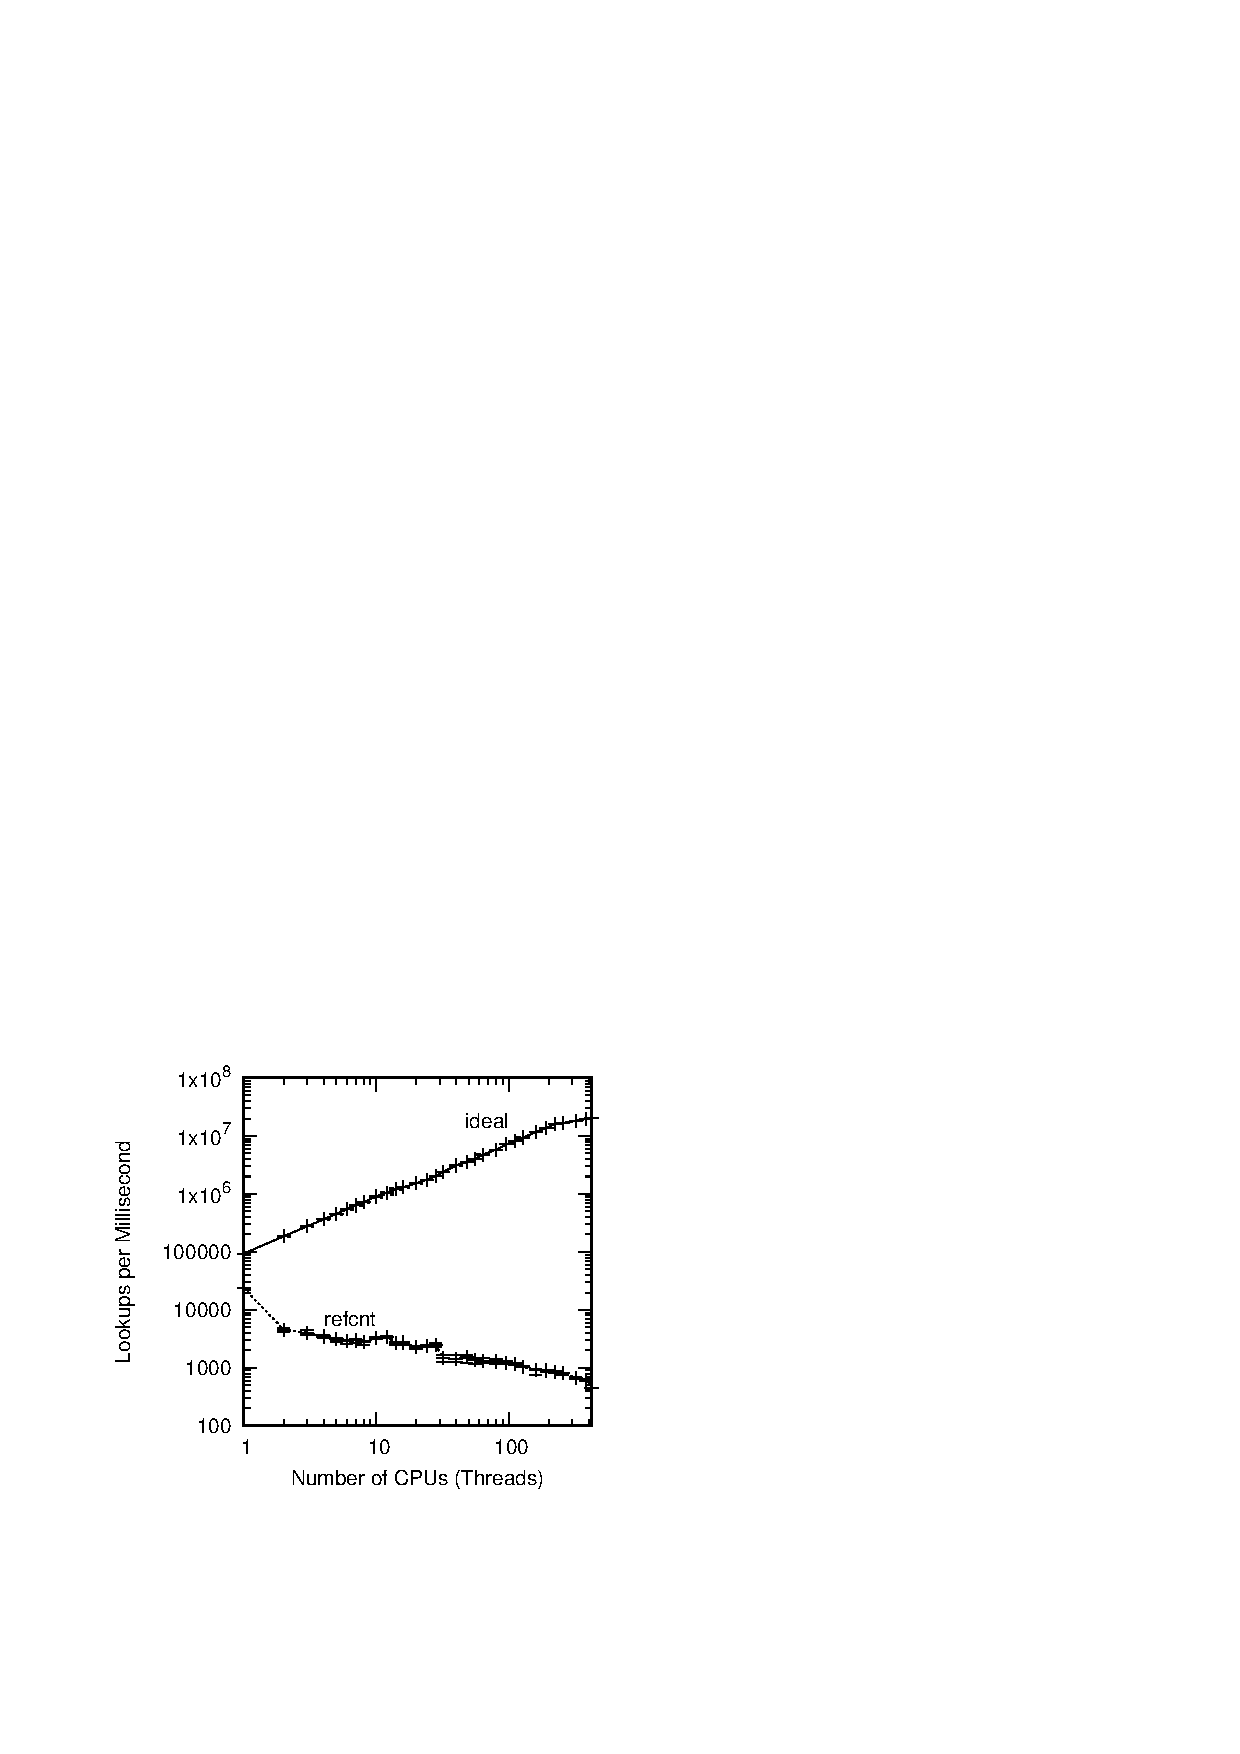
\includegraphics{CodeSamples/defer/perf-refcnt-logscale}}
\caption{Pre-BSD Routing Table Protected by Reference Counting, Log Scale}
\label{fig:defer:Pre-BSD Routing Table Protected by Reference Counting, Log Scale}
\end{figure}

	Figure~\ref{fig:defer:Pre-BSD Routing Table Protected by Reference Counting, Log Scale}
	는 같은 데이터를 로그-로그 플랏 (log-log plot) 으로 보입니다.
	볼 수 있듯, refcnt 라인은 두개 CPU 에서 5,000 아래로 떨어집니다.
	이는 두개 CPU 에서의 이 refcnt 성능은
	Figure~\ref{fig:defer:Pre-BSD Routing Table Protected by Reference Counting}
	에서의 첫번째 y-axis tick 인 $5 \times 10^6$ 보다 천배 이상 적음을
	의미합니다.
	따라서,
	Figure~\ref{fig:defer:Pre-BSD Routing Table Protected by Reference Counting}
	에 보인 레퍼런스 카운팅의 성능 묘사는 너무나도 정확합니다.

	\iffalse

	Figure~\ref{fig:defer:Pre-BSD Routing Table Protected by Reference Counting, Log Scale}
	shows the same data, but on a log-log plot.
	As you can see, the refcnt line drops below 5,000 at two CPUs.
	This means that the refcnt performance at two CPUs is more than
	one thousand times smaller than the first y-axis tick of
	$5 \times 10^6$ in
	Figure~\ref{fig:defer:Pre-BSD Routing Table Protected by Reference Counting}.
	Therefore, the depiction of the performance of reference counting
	shown in
	Figure~\ref{fig:defer:Pre-BSD Routing Table Protected by Reference Counting}
	is all too accurate.

	\fi

}\QuickQuizEndE
}

하지만 이건 심지어 더 나빠집니다.

반복적으로 \co{route_add()} 와 \co{route_del()} 을 호출하는 여러 업데이터
쓰레드를 수행시키는 것은 금방
Listing~\ref{lst:defer:Reference-Counted Pre-BSD Routing Table Lookup} 의
line~\ref{ln:defer:route_refcnt:lookup:lookup:abort}  에 있는 메모리 해제 후
사용 버그를 알리는 \co{abort()} 문을 수행되게 합니다.
이는 곧 레퍼런스 카운트는 확장성과 성능을 저하시킬 뿐만 아니라 필요한 보호를
제공하는데도 실패함을 의미합니다.

Figure~\ref{fig:defer:Pre-BSD Packet Routing List} 에 보인 리스트로 보이는 이
메모리 해제 후 사용 버그를 일으키는 순차적 이벤트 중 하나는 다음과 같습니다:

\iffalse

But it gets worse.

Running multiple updater threads repeatedly invoking
\co{route_add()} and \co{route_del()} will quickly encounter the
\co{abort()} statement on
line~\ref{ln:defer:route_refcnt:lookup:lookup:abort} of
Listing~\ref{lst:defer:Reference-Counted Pre-BSD Routing Table Lookup},
which indicates a use-after-free bug.
This in turn means that the reference counts are not only profoundly
degrading scalability and performance, but also failing to provide
the needed protection.

One sequence of events leading to the use-after-free bug is as follows,
given the list shown in
Figure~\ref{fig:defer:Pre-BSD Packet Routing List}:

\fi

\begin{fcvref}[ln:defer:route_refcnt:lookup]
\begin{enumerate}
\item	쓰레드~A 가 주소~42 를 탐색하여,
	Listing~\ref{lst:defer:Reference-Counted Pre-BSD Routing Table Lookup}
	의 \co{route_lookup()} 의 라인~\lnref{lookup:check_NULL} 에 도달합니다.
	달리 말하자면, 쓰레드~A 는 첫번째 원소로의 포인터를 갖지만, 아직
	그것으로의 참조는 획득하지 않았습니다.
\item	쓰레드~B 가 주소~42 의 route 원소를 제거하기 위해
	Listing~\ref{lst:defer:Reference-Counted Pre-BSD Routing Table Add/Delete}
	의 \co{route_del()} 을 호출합니다.
	이는 성공적으로 마무리 되며, 이 원소의 \co{->re_refcnt} 필드는 값 1을
	가졌으므로 \co{->re_freed} 필드를 설정하고 이 원소를 메모리 해제하기
	위해 \co{re_free()} 를 호출합니다.
\item	쓰레드~A 는 \co{route_lookup()} 의 수행을 계속합니다.
	\co{rep} 포인터는 \co{NULL} 이 아니지만, 라인~\lnref{lookup:check_uaf}
	는 그 \co{->re_freed} 필드가 0이 아님을 보게 되므로,
	라인~\lnref{lookup:abort} 는 \co{abort()} 를 호출합니다.

\iffalse

\item	Thread~A looks up address~42, reaching
	line~\lnref{lookup:check_NULL} of
	\co{route_lookup()} in
	Listing~\ref{lst:defer:Reference-Counted Pre-BSD Routing Table Lookup}.
	In other words, Thread~A has a pointer to the first element,
	but has not yet acquired a reference to it.
\item	Thread~B invokes \co{route_del()} in
	Listing~\ref{lst:defer:Reference-Counted Pre-BSD Routing Table Add/Delete}
	to delete the route entry for address~42.
	It completes successfully, and because this entry's \co{->re_refcnt}
	field was equal to the value one, it invokes
	\co{re_free()} to set the \co{->re_freed} field and to free the entry.
\item	Thread~A continues execution of \co{route_lookup()}.
	Its \co{rep} pointer is non-\co{NULL}, but
	line~\lnref{lookup:check_uaf} sees that
	its \co{->re_freed} field is non-zero,
        so line~\lnref{lookup:abort} invokes
	\co{abort()}.

\fi

\end{enumerate}
\end{fcvref}

문제는 이 레퍼런스 카운트가 보호되어야 할 객체 내에 위치해 있지만, 이는 이
레퍼런스 카운트 자체가 획득되는 그 순간에는 보호가 없음을 의미합니다!
이는 Gamsa 등~\cite{Gamsa99} 에 의해 이야기된 레퍼런스 카운팅에 대비되는 락킹
문제입니다.
어떤 사람은 route 원소별 레퍼런스 카운트 획득을 보호하기 위한 글로벌 락이나
레퍼런스 카운트를 상상해 볼 수 있겠지만, 이는 상당한 컨텐션 문제를 일으킬
겁니다.
동시적 환경에서 안전한 레퍼런스 카운트 획득을 허용하는 알고리즘이
존재하지만~\cite{Valois95a}, 그것들은 극단적으로 복잡하고 에러에 취약할 뿐
아니라~\cite{MagedMichael95a}, 처참한 성능과 확장성을
제공합니다~\cite{ThomasEHart2007a}.

짧게 요약하자면, 동시성은 레퍼런스 카운팅의 유용성을 분명 줄였습니다!

\iffalse

The problem is that the reference count is located in the object
to be protected, but that means that there is no protection during
the instant in time when the reference count itself is being acquired!
This is the reference-counting counterpart of a locking issue noted
by Gamsa et al.~\cite{Gamsa99}.
One could imagine using a global lock or reference count to protect
the per-route-entry reference-count acquisition, but this would
result in severe contention issues.
Although algorithms exist that allow safe reference-count acquisition
in a concurrent environment~\cite{Valois95a}, they are not only extremely
complex and error-prone~\cite{MagedMichael95a}, but also provide
terrible performance and scalability~\cite{ThomasEHart2007a}.

In short, concurrency has most definitely reduced the usefulness
of reference counting!

\fi

\QuickQuiz{
	동시성이 ``레퍼런스 카운팅의 유용성을 분명 줄였다'' 면, 리눅스 커널에는
	왜 그렇게 많은 레퍼런스 카운터가 존재하나요?

	\iffalse

	If concurrency has ``most definitely reduced the usefulness
	of reference counting'', why are there so many reference
	counters in the Linux kernel?

	\fi

}\QuickQuizAnswer{
	해당 문장은 ``유용성을 줄였다'' 고 했지, ``유용성을 제거했다'' 고는
	하지 않았죠?

	리눅스 커널이 상당히 동시적인 환경에서 레퍼런스 카운팅의 장점을 취하기
	위해 사용하는 기법들 중 일부를 이야기 하는
	Section~\ref{sec:together:Refurbish Reference Counting} 를 보시기
	바랍니다.

	\iffalse

	That sentence did say ``reduced the usefulness'', not
	``eliminated the usefulness'', now didn't it?

	Please see
	Section~\ref{sec:together:Refurbish Reference Counting},
	which discusses some of the techniques that the Linux kernel
	uses to take advantage of reference counting in a highly
	concurrent environment.

	\fi

}\QuickQuizEnd

그렇다고는 하나, 때로는 어떤 문제를 해결하기 위해선 그걸 완전 다른 방식으로 볼
필요가 있습니다.
다음 섹션은 훌륭한 성능과 확장성을 제공하는 안에서 바깥으로 향하는 레퍼런스
카운트로 생각 될 수 있는 방법을 알아보겠습니다.

\iffalse

That said, sometimes it is necessary to look at a problem in an
entirely different way in order to successfully solve it.
The next section describes what could be thought of as an
inside-out reference count that provides decent performance
and scalability.

\fi
